
\begin{figure}
\centering

% Define block styles used later

\tikzstyle{module}=[draw, draw=blue!80, text width=10em, 
    text centered, minimum height=5em, minimum width = 10em, drop shadow, rounded corners,
    fill=blue!30]
    
\tikzstyle{vecArrow} = [thick, decoration={markings,mark=at position
   1 with {\arrow[semithick]{open triangle 60}}},
   double distance=1.4pt, shorten >= 5.5pt,
   preaction = {decorate},
   postaction = {draw,line width=1.4pt, white,shorten >= 4.5pt}]

% Define distances for bordering
\def\blockdist{1.5}
\def\edgedist{2.5}

\definecolor{darkblue}{rgb}{0.2,0.2,0.6}
\definecolor{darkred}{rgb}{0.6,0.1,0.1}
\definecolor{darkgreen}{rgb}{0.2,0.6,0.2}

\def\arrow{
  (10.75:1.1) -- (6.5:1) arc (6.25:120:1) [rounded corners=0.5] --
  (120:0.9) [rounded corners=1] -- (130:1.1) [rounded corners=0.5] --
  (120:1.3) [sharp corners] -- (120:1.2) arc (120:5.25:1.2)
  [rounded corners=1] -- (10.75:1.1) -- (6.5:1) -- cycle
}

\tikzset{
  ashadow/.style={opacity=.25, shadow xshift=0.07, shadow yshift=-0.07},
}

\def\arrows[#1]{         
  \begin{scope}[scale=#1]
	\node[align=center] at (0,0) {\Huge{ Loop } \\ \Huge{ until matching } };  
  
    \draw[color=darkred, %
    drop shadow={ashadow, color=red!60!black}] \arrow;

    \draw[color=darkgreen, bottom color=green!60!black, top color=green!30, %
    drop shadow={ashadow, color=green!60!black}] [rotate=120] \arrow;

    \draw[color=darkblue, right color=blue!60, left color=blue!30, %
    drop shadow={ashadow, color=blue!60!black}] [rotate=240] \arrow;

    % to hide the green shadow
    \draw[color=darkred, left color=red!60, right color=red!30] \arrow;
  \end{scope}
}

%\begin{tikzpicture}[node distance=3cm,thick,path image/.style={
\begin{tikzpicture}[node distance=3cm,thick,scale=0.5, every node/.style={scale=0.5},path image/.style={
path picture={
\node at (path picture bounding box.center) {
\includegraphics[width=1cm]{#1}
};}}]
\tikzstyle{conefill} = [path image=,fill opacity=0.8]

\node (t2w) at (0,0)	{
\includegraphics[width=1.5cm]{2_modality/figures/tikzimage/dce.eps}};
\begin{scope}[node distance=1.2cm]
\node[below of=t2w] (cap1) {\Large Fixed};
\end{scope}
\begin{scope}[node distance=6cm]
\node[below of=t2w] 	(dce) 			{\includegraphics[width=1.5cm]{2_modality/figures/tikzimage/t2.eps}};
\begin{scope}[node distance=1.2cm]
\node[below of=dce] (cap2) {\Large Moving};
\end{scope}
\end{scope}

\begin{scope}[node distance=5.5cm]
	\node[module,right of=t2w] (sim) {\Large Similarity \\ measure};
\end{scope}
\begin{scope}[node distance=3cm]
	\node[module,below of=sim] (int) {\Large Interpolator};
	\node[module,below of=int] (tra) {\Large Transform};
\end{scope}

\draw[line width=1mm,draw=blue!30,->] (t2w)--(sim);  
\draw[line width=1mm,draw=blue!30,->] (dce)--(tra); 

\begin{scope}[node distance=9cm]
	\node[module,right of=sim] (opt) {\Large Optimizer};
\end{scope}

\draw[draw=blue,->,line width=.5mm] (tra)--(int);
\draw[draw=blue,->,line width=.5mm] (int)--(sim);
\draw[draw=blue,->,line width=.5mm] (sim)--(opt) node[midway,above] {\Large Similarity} node[midway,below] {\Large metric};
\draw[draw=blue,->,line width=.5mm] (opt)|-(tra); 

\begin{pgfonlayer}{background}
	\path (sim.west |- sim.north)+(-0.5,.5) node (a) {};
    \path (opt.east |- tra.south)+(+0.5,-0.5) node (b) {};
          
    \path[fill=blue!10,rounded corners, draw=blue!20, dashed] (a) rectangle (b);
\end{pgfonlayer} 

\begin{scope}[node distance=5cm]
\node[right of=int] (arr) {
\begin{tikzpicture}
\arrows[1.9];
\end{tikzpicture}
};
\end{scope}
\end{tikzpicture}
\caption[Registration framework.]{Typical framework involved to solve the registration problem.}
\label{fig:frareg}
\end{figure}



%\tikzset{
%  ashadow/.style={opacity=.25, shadow xshift=0.07, shadow yshift=-0.07},
%}
%
%\def\arrows[#1]{         
%  \begin{scope}[scale=#1]
%	\node[align=center] at (0,0) {Loop \\ until \\ matching};  
%  
%    \draw[color=darkred, %
%    drop shadow={ashadow, color=red!60!black}] \arrow;
%
%    \draw[color=darkgreen, bottom color=green!60!black, top color=green!30, %
%    drop shadow={ashadow, color=green!60!black}] [rotate=120] \arrow;
%
%    \draw[color=darkblue, right color=blue!60, left color=blue!30, %
%    drop shadow={ashadow, color=blue!60!black}] [rotate=240] \arrow;
%
%    % to hide the green shadow
%    \draw[color=darkred, left color=red!60, right color=red!30] \arrow;
%  \end{scope}
%}
%
%\begin{tikzpicture}[node distance=3cm,thick,path image/.style={
%path picture={
%\node at (path picture bounding box.center) {
%\includegraphics[width=.5cm]{#1}
%};}}]
%\tikzstyle{conefill} = [path image=,fill opacity=0.8]
%
%\node[inner sep=0pt] (t2w) at (0,0)	{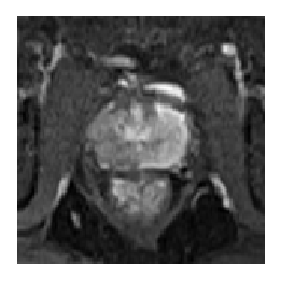
\includegraphics[width=1cm]{02_background/figures/tikzimage/dce.eps}};
%\begin{scope}[node distance=.8cm]
%\node[below of=t2w] (cap1) {Fixed};
%\end{scope}
%\begin{scope}[node distance=3.5cm]
%\node[below of=t2w] 	(dce) 			{\includegraphics[width=1cm]{02_background/figures/tikzimage/t2.eps}};
%\begin{scope}[node distance=.8cm]
%\node[below of=dce] (cap2) {Moving};
%\end{scope}
%\end{scope}
%
%\begin{scope}[node distance=2.5cm]
%	\node[module,right of=t2w] (sim) {Similarity \\ measure};
%\end{scope}
%\begin{scope}[node distance=1.75cm]
%	\node[module,below of=sim] (int) {Interpolator};
%	\node[module,below of=int] (tra) {Transform};
%\end{scope}
%\begin{scope}[node distance=5cm]
%	\node[module,right of=sim] (opt) {Optimizer};
%\end{scope}
%
%\draw[draw=blue,->,line width=.5mm] (tra)--(int);
%\draw[draw=blue,->,line width=.5mm] (int)--(sim);
%\draw[draw=blue,->,line width=.5mm] (sim)--(opt) node[midway,above] {Similarity} node[midway,below] {metric};
%\draw[draw=blue,->,line width=.5mm] (opt)|-(tra);
%
%\draw[line width=.8mm,draw=blue!30,->] (t2w)--(sim);  
%\draw[line width=.8mm,draw=blue!30,->] (dce)--(tra);  
%
%\begin{pgfonlayer}{background}
%	\path (sim.west |- sim.north)+(-0.3,.3) node (a) {};
%    \path (opt.east |- tra.south)+(+0.3,-0.3) node (b) {};
%          
%    \path[fill=blue!10,rounded corners, draw=blue!20, dashed] (a) rectangle (b);
%\end{pgfonlayer} 
%
%\begin{scope}[node distance=3cm]
%\node[right of=int] (arr) {
%\begin{tikzpicture}
%\arrows[1];
%\end{tikzpicture}
%};
%\end{scope}
